% Options for packages loaded elsewhere
\PassOptionsToPackage{unicode}{hyperref}
\PassOptionsToPackage{hyphens}{url}
%
\documentclass[
  10pt,
  a4paper,
]{article}
\usepackage{amsmath,amssymb}
\usepackage{iftex}
\ifPDFTeX
  \usepackage[T1]{fontenc}
  \usepackage[utf8]{inputenc}
  \usepackage{textcomp} % provide euro and other symbols
\else % if luatex or xetex
  \usepackage{unicode-math} % this also loads fontspec
  \defaultfontfeatures{Scale=MatchLowercase}
  \defaultfontfeatures[\rmfamily]{Ligatures=TeX,Scale=1}
\fi
\usepackage{lmodern}
\ifPDFTeX\else
  % xetex/luatex font selection
  \setmainfont[]{Noto Serif CJK JP}
  \setsansfont[]{Noto Sans CJK JP}
  \setmonofont[]{Noto Sans Mono CJK JP}
\fi
% Use upquote if available, for straight quotes in verbatim environments
\IfFileExists{upquote.sty}{\usepackage{upquote}}{}
\IfFileExists{microtype.sty}{% use microtype if available
  \usepackage[]{microtype}
  \UseMicrotypeSet[protrusion]{basicmath} % disable protrusion for tt fonts
}{}
\makeatletter
\@ifundefined{KOMAClassName}{% if non-KOMA class
  \IfFileExists{parskip.sty}{%
    \usepackage{parskip}
  }{% else
    \setlength{\parindent}{0pt}
    \setlength{\parskip}{6pt plus 2pt minus 1pt}}
}{% if KOMA class
  \KOMAoptions{parskip=half}}
\makeatother
\usepackage{xcolor}
\usepackage[margin=22mm]{geometry}
\usepackage{color}
\usepackage{fancyvrb}
\newcommand{\VerbBar}{|}
\newcommand{\VERB}{\Verb[commandchars=\\\{\}]}
\DefineVerbatimEnvironment{Highlighting}{Verbatim}{commandchars=\\\{\}}
% Add ',fontsize=\small' for more characters per line
\newenvironment{Shaded}{}{}
\newcommand{\AlertTok}[1]{\textcolor[rgb]{1.00,0.00,0.00}{\textbf{#1}}}
\newcommand{\AnnotationTok}[1]{\textcolor[rgb]{0.38,0.63,0.69}{\textbf{\textit{#1}}}}
\newcommand{\AttributeTok}[1]{\textcolor[rgb]{0.49,0.56,0.16}{#1}}
\newcommand{\BaseNTok}[1]{\textcolor[rgb]{0.25,0.63,0.44}{#1}}
\newcommand{\BuiltInTok}[1]{\textcolor[rgb]{0.00,0.50,0.00}{#1}}
\newcommand{\CharTok}[1]{\textcolor[rgb]{0.25,0.44,0.63}{#1}}
\newcommand{\CommentTok}[1]{\textcolor[rgb]{0.38,0.63,0.69}{\textit{#1}}}
\newcommand{\CommentVarTok}[1]{\textcolor[rgb]{0.38,0.63,0.69}{\textbf{\textit{#1}}}}
\newcommand{\ConstantTok}[1]{\textcolor[rgb]{0.53,0.00,0.00}{#1}}
\newcommand{\ControlFlowTok}[1]{\textcolor[rgb]{0.00,0.44,0.13}{\textbf{#1}}}
\newcommand{\DataTypeTok}[1]{\textcolor[rgb]{0.56,0.13,0.00}{#1}}
\newcommand{\DecValTok}[1]{\textcolor[rgb]{0.25,0.63,0.44}{#1}}
\newcommand{\DocumentationTok}[1]{\textcolor[rgb]{0.73,0.13,0.13}{\textit{#1}}}
\newcommand{\ErrorTok}[1]{\textcolor[rgb]{1.00,0.00,0.00}{\textbf{#1}}}
\newcommand{\ExtensionTok}[1]{#1}
\newcommand{\FloatTok}[1]{\textcolor[rgb]{0.25,0.63,0.44}{#1}}
\newcommand{\FunctionTok}[1]{\textcolor[rgb]{0.02,0.16,0.49}{#1}}
\newcommand{\ImportTok}[1]{\textcolor[rgb]{0.00,0.50,0.00}{\textbf{#1}}}
\newcommand{\InformationTok}[1]{\textcolor[rgb]{0.38,0.63,0.69}{\textbf{\textit{#1}}}}
\newcommand{\KeywordTok}[1]{\textcolor[rgb]{0.00,0.44,0.13}{\textbf{#1}}}
\newcommand{\NormalTok}[1]{#1}
\newcommand{\OperatorTok}[1]{\textcolor[rgb]{0.40,0.40,0.40}{#1}}
\newcommand{\OtherTok}[1]{\textcolor[rgb]{0.00,0.44,0.13}{#1}}
\newcommand{\PreprocessorTok}[1]{\textcolor[rgb]{0.74,0.48,0.00}{#1}}
\newcommand{\RegionMarkerTok}[1]{#1}
\newcommand{\SpecialCharTok}[1]{\textcolor[rgb]{0.25,0.44,0.63}{#1}}
\newcommand{\SpecialStringTok}[1]{\textcolor[rgb]{0.73,0.40,0.53}{#1}}
\newcommand{\StringTok}[1]{\textcolor[rgb]{0.25,0.44,0.63}{#1}}
\newcommand{\VariableTok}[1]{\textcolor[rgb]{0.10,0.09,0.49}{#1}}
\newcommand{\VerbatimStringTok}[1]{\textcolor[rgb]{0.25,0.44,0.63}{#1}}
\newcommand{\WarningTok}[1]{\textcolor[rgb]{0.38,0.63,0.69}{\textbf{\textit{#1}}}}
\usepackage{longtable,booktabs,array}
\usepackage{calc} % for calculating minipage widths
% Correct order of tables after \paragraph or \subparagraph
\usepackage{etoolbox}
\makeatletter
\patchcmd\longtable{\par}{\if@noskipsec\mbox{}\fi\par}{}{}
\makeatother
% Allow footnotes in longtable head/foot
\IfFileExists{footnotehyper.sty}{\usepackage{footnotehyper}}{\usepackage{footnote}}
\makesavenoteenv{longtable}
\usepackage{graphicx}
\makeatletter
\def\maxwidth{\ifdim\Gin@nat@width>\linewidth\linewidth\else\Gin@nat@width\fi}
\def\maxheight{\ifdim\Gin@nat@height>\textheight\textheight\else\Gin@nat@height\fi}
\makeatother
% Scale images if necessary, so that they will not overflow the page
% margins by default, and it is still possible to overwrite the defaults
% using explicit options in \includegraphics[width, height, ...]{}
\setkeys{Gin}{width=\maxwidth,height=\maxheight,keepaspectratio}
% Set default figure placement to htbp
\makeatletter
\def\fps@figure{htbp}
\makeatother
\setlength{\emergencystretch}{3em} % prevent overfull lines
\providecommand{\tightlist}{%
  \setlength{\itemsep}{0pt}\setlength{\parskip}{0pt}}
\setcounter{secnumdepth}{5}
\usepackage{setspace}
\setstretch{1.15}
\usepackage{needspace,etoolbox}
\pretocmd{\section}{\Needspace{8\baselineskip}}{}{}
\pretocmd{\subsection}{\Needspace{6\baselineskip}}{}{}
\XeTeXlinebreaklocale "ja"
\XeTeXlinebreakskip=0pt plus 1pt
\setlength{\parindent}{1em}
\setlength{\parskip}{0.35em}
\renewcommand{\arraystretch}{1.15}
\usepackage{fvextra}
\DefineVerbatimEnvironment{Highlighting}{Verbatim}{breaklines,commandchars=\\\{\}}
\renewcommand{\CommentTok}[1]{\textcolor[rgb]{0.25,0.25,0.25}{#1}}
\ifLuaTeX
  \usepackage{selnolig}  % disable illegal ligatures
\fi
\usepackage{bookmark}
\IfFileExists{xurl.sty}{\usepackage{xurl}}{} % add URL line breaks if available
\urlstyle{same}
\hypersetup{
  pdftitle={枝刈り・CSRによる色補正モデルの圧縮},
  pdfauthor={25G1017　岩澤大心},
  hidelinks,
  pdfcreator={LaTeX via pandoc}}

\title{枝刈り・CSRによる色補正モデルの圧縮}
\usepackage{etoolbox}
\makeatletter
\providecommand{\subtitle}[1]{% add subtitle to \maketitle
  \apptocmd{\@title}{\par {\large #1 \par}}{}{}
}
\makeatother
\subtitle{アジャイルワーク2　実験報告書}
\author{25G1017　岩澤大心}
\date{記録整理日：2026年11月13日}

\begin{document}
\maketitle

\section{概要}\label{ux6982ux8981}

色補正ニューラルネットワークに枝刈りとCSRを適用し，Denseと容量・推論時間・MSEを比較した．隠れ層の大きさHを40・60・80・100とし，9色のチャートを10回読み取った．各回の同じ入力を全8条件へ与えた．

モデル配列容量は60.51〜69.70\%，固定入力による実機推論時間は28.97〜44.01\%，単独モデル入りプログラムのFlashは7.94〜31.26\%減少した．静的RAMは全8条件で6,764
byteだった．一方，10回平均MSEはDenseが231.68〜319.56，枝刈り＋CSRが452.04〜651.92となり，容量・速度の改善と精度維持の両立は達成しなかった．

\section{目的}\label{ux76eeux7684}

Arduino上の色補正モデルについて，枝刈り＋CSRによる保存容量と推論時間の削減効果，および補正精度への影響を調べる．Denseに対するMSE増加5\%以下を精度維持の条件とし，MSE300以下も別に判定する．

同じHのDenseと枝刈り＋CSRへ同一入力を与えて比較した．当初計画の40・50・60次元から，実施条件を40・60・80・100へ変更した．H50は未実施である．

\section{比較の構成}\label{ux6bd4ux8f03ux306eux69cbux6210}

図1のように，1回のセンサ読取から得たRGBを両方式へ入力した．4種類のHと2方式を組み合わせ，比較条件は8個とした．

\Needspace{14\baselineskip}

\noindent\begin{minipage}{\linewidth}

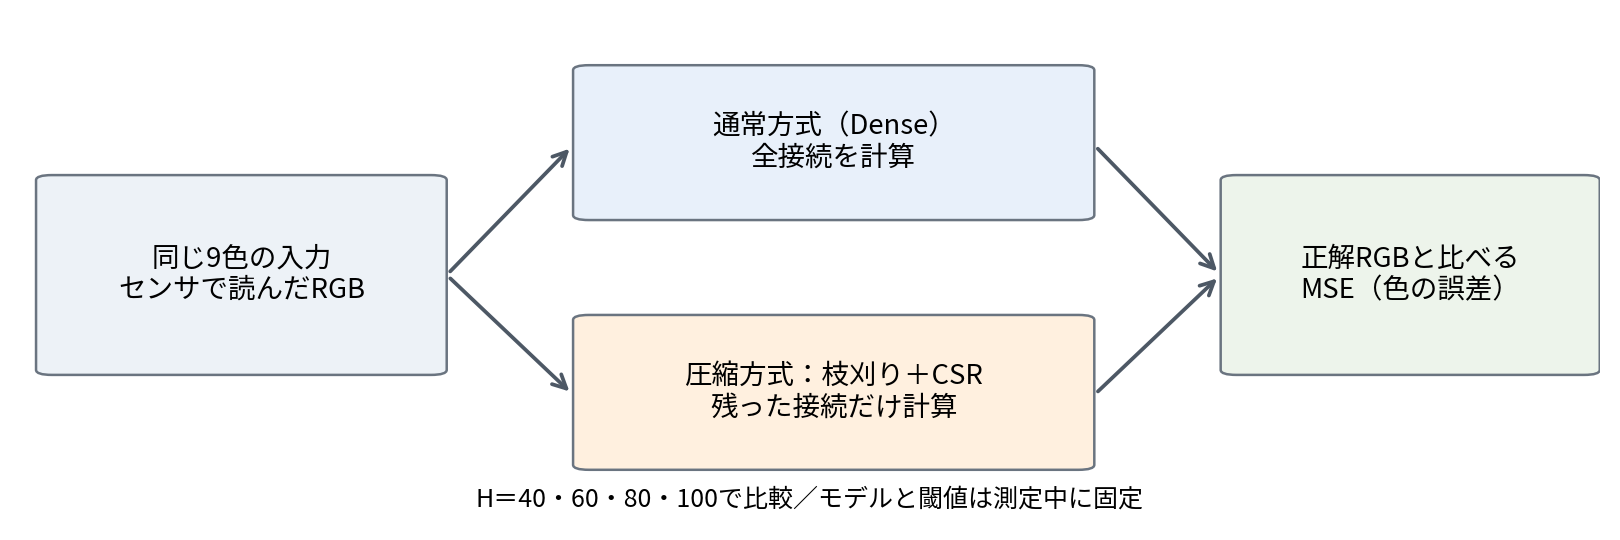
\includegraphics{figures/comparison_flow.png}

\begingroup\centering\setlength{\parindent}{0pt}

図1　同一入力による比較

\par\endgroup

\end{minipage}

\begin{longtable}[]{@{}ll@{}}
\toprule\noalign{}
用途 & データ・操作 \\
\midrule\noalign{}
\endhead
\bottomrule\noalign{}
\endlastfoot
学習 & 過去の実測135行：3×3チャート111行，6×4チャート24行 \\
閾値選択 & 別の8×8チャートを2回読んだ128入力と，学習内9入力 \\
精度測定 & 学習にも使用した3×3チャートを新しく10回読取，計90入力 \\
速度測定 & 保存済み実測9入力を実機で反復再生 \\
メモリ比較 & 各モデル単独の8条件をコンパイル \\
\end{longtable}

新規10回の入力は学習・閾値選択へ加えていない．ただし，色自体は学習時と同じであり，独立した未見チャートによる最終評価ではない．

\section{仕組みと計算方法}\label{ux4ed5ux7d44ux307fux3068ux8a08ux7b97ux65b9ux6cd5}

\subsection{ネットワークと学習}\label{ux30cdux30c3ux30c8ux30efux30fcux30afux3068ux5b66ux7fd2}

ネットワークは3−H−H−3の全結合構造とした．入力を
\(\boldsymbol x\)，重みを \(W\)，バイアスを \(\boldsymbol b\) とすると，

\[
\begin{aligned}
\boldsymbol h_1&=\operatorname{ReLU}(W_1\boldsymbol x+\boldsymbol b_1),\\
\boldsymbol h_2&=\operatorname{ReLU}(W_2\boldsymbol h_1+\boldsymbol b_2),\\
\boldsymbol y&=W_3\boldsymbol h_2+\boldsymbol b_3.
\end{aligned}
\]

隠れ層にReLUを用い，出力層は線形とした．学習には，重み付きSmooth
L1損失{[}5{]}と，バイアスを除く重みへのL1正則化{[}1{]}を用いた．

\[
\mathcal L=\frac{1}{\sum_{i=1}^{M}a_i}
\sum_{i=1}^{M}\frac{a_i}{3}\sum_{c\in\{R,G,B\}}
\ell_\beta(\widehat y_{i,c}-t_{i,c})
+10^{-6}\sum_{\ell=1}^{3}\sum_{j,k}|(W_\ell)_{jk}|,
\]

\[
\ell_\beta(e)=\begin{cases}e^2/(2\beta)&(|e|<\beta),\\|e|-\beta/2&(|e|\geq\beta),\end{cases}\qquad \beta=0.05
\]

\(M=135\) は学習行数，\(a_i>0\) は行ごとの重要度，\(\widehat y\)
は予測，\(t\) は正解，\(c\)
はRGB成分を表す．学習時の尺度は0〜1とした．\(\ell\)
は層番号，jとkは行列内の位置である．L1項は全3層の重みの絶対値を合計し，小さい重みを作る方向に作用する．学習損失と，評価時の整数RGBのMSEは区別する．

\subsection{枝刈りとCSR}\label{ux679dux5208ux308aux3068csr}

枝刈り{[}2{]}では \(|w|<\tau\)
の重みを0にし，バイアスは保持した．残った重みを，値・列番号・行開始位置の3配列からなるCSR{[}3{]}へ変換した．保存・計算対象を非ゼロ重みに限定する．3層の非ゼロ重み数をKとすると，疎性Sは次式である．

\[S=1-\frac{K}{H^2+6H}\]

\subsection{メモリ容量の手計算}\label{ux30e1ux30e2ux30eaux5bb9ux91cfux306eux624bux8a08ux7b97}

Denseの重み数は \(N_w=3H+H^2+3H\)，バイアス数は \(N_b=2H+3\)
である．FP32は1個4 byteなので，

\[B_{\mathrm{Dense}}=4(N_w+N_b)=4(H^2+8H+3)\quad[\mathrm{byte}]\]

となる．CSRは非ゼロ重みK個をFP32，列番号をuint8，行開始位置をuint16で保存する．行位置は3層の行数に各終端を加えた
\(2H+6\) 個となる．バイアスを全て残すと，

\[
\begin{aligned}
B_{\mathrm{CSR}}&=4K+K+2(2H+6)+4(2H+3)\\
&=5K+12H+24\quad[\mathrm{byte}]
\end{aligned}
\]

H60では重み3,960個，バイアス123個，枝刈り後K=1,141個なので，

\[
\begin{aligned}
B_{\mathrm{Dense}}&=4(60^2+8\cdot60+3)=16,332,\\
B_{\mathrm{CSR}}&=4,564+1,141+252+492=6,449,\\
R_B&=100(1-6,449/16,332)=60.51\%
\end{aligned}
\]

\Needspace{10\baselineskip}

全HのCSR配列の内訳を示す．単位はbyteである．

\begin{longtable}[]{@{}lrrrrr@{}}
\toprule\noalign{}
H & 非ゼロ重み & 列番号 & 行位置 & バイアス & 合計byte \\
\midrule\noalign{}
\endhead
\bottomrule\noalign{}
\endlastfoot
40 & 1,880 & 470 & 172 & 332 & 2,854 \\
60 & 4,564 & 1,141 & 252 & 492 & 6,449 \\
80 & 6,596 & 1,649 & 332 & 652 & 9,229 \\
100 & 9,496 & 2,374 & 412 & 812 & 13,094 \\
\end{longtable}

配列容量が減る条件は \(5K<4H^2+20H-12\)
で，採用した4条件は全て満たす．この計算は数値配列のみを対象とし，構造体・アラインメント・Arduinoコア等を含むFlash全体はIDE表示で別に評価した．

\subsection{評価指標}\label{ux8a55ux4fa1ux6307ux6a19}

出力を0〜1へクリップし，255倍して四捨五入した整数RGBで評価した．9色の補正値
\(y\) と正解 \(t\) から，MSEを次式で求めた．

\[\mathrm{MSE}=\frac{1}{27}\sum_{i=1}^{9}\sum_{c\in\{R,G,B\}}(y_{i,c}-t_{i,c})^2\]

\Needspace{6\baselineskip}

各回のMSEを \(m_r\) とし，10回平均と標本標準偏差（SD）を算出した．

\[\overline m=\frac1{10}\sum_{r=1}^{10}m_r,\qquad
s_m=\sqrt{\frac1{9}\sum_{r=1}^{10}(m_r-\overline m)^2}\]

MSE・標本SD・対応差は小数第2位まで表示し，第3位以降を切り捨てる．集計・増加率の計算には切り捨て前の値を使用する．

同じ回の差を \(d_r=m_{r,\mathrm{CSR}}-m_{r,\mathrm{Dense}}\)
とした．MSE増加率は
\(100(\overline m_{\mathrm{CSR}}/\overline m_{\mathrm{Dense}}-1)\)
とし，各回の割合の平均は使わない．容量Bと時間Tの削減率は，それぞれ
\(100(1-B_{\mathrm{CSR}}/B_{\mathrm{Dense}})\)，\(100(1-T_{\mathrm{CSR}}/T_{\mathrm{Dense}})\)
で求めた．

\section{実験方法}\label{ux5b9fux9a13ux65b9ux6cd5}

独立変数はHと方式，従属変数はMSE・モデル配列容量・Flash・静的RAM・推論時間とした．同じHでは，元モデル・入力・RGB丸め・ボード・計時条件をそろえた．H間では追加学習前の重みも異なる．

\subsection{装置と実行環境}\label{ux88c5ux7f6eux3068ux5b9fux884cux74b0ux5883}

\begin{longtable}[]{@{}
  >{\raggedright\arraybackslash}p{(\columnwidth - 2\tabcolsep) * \real{0.5000}}
  >{\raggedright\arraybackslash}p{(\columnwidth - 2\tabcolsep) * \real{0.5000}}@{}}
\toprule\noalign{}
\begin{minipage}[b]{\linewidth}\raggedright
項目
\end{minipage} & \begin{minipage}[b]{\linewidth}\raggedright
実施条件
\end{minipage} \\
\midrule\noalign{}
\endhead
\bottomrule\noalign{}
\endlastfoot
ボード & Arduino UNO R4 WiFi \\
主マイコン・クロック & Renesas RA4M1，48 MHz \\
公称Flash／SRAM & 262,144／32,768 byte \\
センサ & A0へ接続した光センサ，型番未確認 \\
LED & R:D8，G:D6，B:D7，analogWrite 255／0 \\
読取設定 & 各チャンネル10サンプル平均，サンプル間2 ms，点灯後10
ms待機 \\
操作 & シリアル9600 bps，外付けD2/D3ボタンは不使用 \\
PC環境 & Mac，Jupyter Notebook \\
最終学習・集計 & クラウドPython 3.12，PyTorch 2.8.0，NumPy 2.3.5 \\
実機コンパイラ & 7.2.1 20170904，ARM/embedded-7-branch revision
255204 \\
Arduino IDE・コア & 版番号未記録，コンパイラ文字列を保存 \\
\end{longtable}

紙は手で支え，照明を同じ状態に保つ手順で測定した．照度・距離・角度の定量記録はない．

\subsection{学習データと正解画像}\label{ux5b66ux7fd2ux30c7ux30fcux30bfux3068ux6b63ux89e3ux753bux50cf}

実測135行を全て保持し，配布Notebookの見本入力は実測として追加しなかった．正解画像の取り違えを修正し，最終V10では3×3分111行の教師値と評価を，先生指定の元の
\texttt{result.ppm}
へ統一した．灰色の正解は(127,127,127)である．6×4分24行は元のNotebookの教師値を保持したが，別の先生指定PPMとの照合はできていない．旧CMYK基準のMSEは結果へ混在させない．

各Hは同じHのV9重みから40,000
epoch追加学習した．seed42，Adam，cosine学習率0.0005→0.000005とし，色・校正グループや過去入力の整合度に基づく正の行重要度を使用した．

データ拡張として，3×3入力の50\%にRGB別gain
0.75〜1.30とoffsetを加えた．灰・白には30\%の確率で共通gain
0.5〜1.15を適用した．offset幅は学習入力間の距離から定め，設定と行重要度をコード・CSVへ保存した．これは学習時の変換であり，物理測定の追加ではない．

\subsection{実装アルゴリズムとソースコード}\label{ux5b9fux88c5ux30a2ux30ebux30b4ux30eaux30baux30e0ux3068ux30bdux30fcux30b9ux30b3ux30fcux30c9}

PCで学習・閾値選択・枝刈り・CSR変換を行い，Dense重みとCSR配列を数値ヘッダへ出力した．Arduinoでは共通入力から両方式を計算した．重みの形式は両方式ともFP32とした．

CSR変換では各層を行順に走査し，非ゼロ重みを \texttt{values}，列番号を
\texttt{col}，各行の開始位置と終端を \texttt{row}
へ格納した．列番号は昇順とし，加算順序を元の行列にそろえた．

\texttt{trained\_models::predict()}
はDenseの3層の推論を行う．\texttt{comparison\_models::sparseLayer()}
はCSR形式の1層を計算し，\texttt{comparison\_models::predict()}
は条件番号に応じてDenseまたは3層のCSR推論を呼び出す．隠れ層のみReLUを適用し，中間値を2本の作業配列へ保持する．

新規読取では \texttt{normalizeInput()}
が黒白校正値による正規化とクリップを行い，\texttt{comparison\_models::inferAll()}
が同一入力から全8条件の出力を求める．\texttt{outputTo255()}
は出力を0〜255の整数へ変換する．整数RGBをPPMとして保存し，正解画像とのMSEを算出する．

\texttt{validIndices()}
で行位置の単調性・終端・列範囲を，\texttt{selfCheckAll()}
で固定入力に対する出力を検査した．CSR変換の正しさは枝刈り後のDense計算と照合し，精度への影響は枝刈り前のDenseとのMSE差で評価した．

学習は \texttt{train.py}，候補比較は
\texttt{select\_compression.py}，追加条件による閾値固定は
\texttt{finalize\_compression.py}，ヘッダ出力は
\texttt{build\_program.py} を使用した．受領ログは
\texttt{record\_fresh\_capture.py}，単独ビルド表示は
\texttt{record\_single\_model\_memory.py} で検算・集計した．

CSR推論と計時の関数は，付録の「コメント付きコード」に行ごとの説明を付して掲載する．

\subsection{閾値選択}\label{ux95beux5024ux9078ux629e}

学習済み重みの絶対値について，隣接する異なる値の中間を候補とし，候補数は固定しなかった．検証128入力でMSE増加5\%以下かつDenseより小容量となり，学習内V8の9入力でもMSE300以下となる候補から最小容量のものを選んだ．新規10回の開始前に重み・閾値を固定した．

下表は選択に使用した入力での結果である．検証2回目には異なる6色が同じ0入力になる問題があり，選択は暫定とした．

\begin{longtable}[]{@{}lrrrr@{}}
\toprule\noalign{}
H & 検証Dense MSE & 検証CSR MSE & 変化率 & 学習内V8の9入力CSR MSE \\
\midrule\noalign{}
\endhead
\bottomrule\noalign{}
\endlastfoot
40 & 5012.20 & 4715.84 & -5.91\% & 277.51 \\
60 & 5226.80 & 5292.58 & +1.26\% & 260.18 \\
80 & 5135.43 & 4553.44 & -11.33\% & 259.25 \\
100 & 5237.21 & 4632.38 & -11.55\% & 290.37 \\
\end{longtable}

\subsection{紙の新規10回読取}\label{ux7d19ux306eux65b0ux898f10ux56deux8aadux53d6}

\texttt{TEACHER\_FRESH\_V10}
で，各回に黒b・白wを登録した．各RGBの読取値vから \((v-b)/(w-b)\)
を求め，0〜1へクリップして入力とした．

赤・緑・青・黄・水色・紫・黒・灰・白の順に紙を当て直し，rを各1回送信した．同じ新規入力を全8モデルへ与え，9色終了後に8個のMSEと8枚のPPMを保存した．nで次回の校正へ進み，CAPTURE=1〜10を実施した．反復単位は9色の読取1回であり，内部10サンプル平均は反復回数に数えない．

RAW・黒白校正値・正規化入力・モデル識別値・閾値・PPMを全回保存した．第2回は高MSEだったが，操作ミスの申告はなく，全10回を集計した．除外した回はない．

\subsection{速度と容量の測定}\label{ux901fux5ea6ux3068ux5bb9ux91cfux306eux6e2cux5b9a}

\texttt{TEACHER\_RESULT\_COMPARE\_V10} の \texttt{timeModel()}
は，指定モデルの推論を保存済み実測9入力で100回行い，\texttt{micros()}
{[}4{]}で経過時間を求める関数である．\texttt{comparison\_models::predict()}
で推論を呼び出し，出力の合計をチェックサムとして保持する．\texttt{runBenchmarks()}
は各モデル10回のウォームアップ後に100推論×5組を計時し，Dense先行とCSR先行を交互にする．経過時間を100で割り，1推論当たりの時間を求めた．

計時区間は推論・入力選択・チェックサム加算を含み，センサ読取・シリアル出力・MSE計算を除く．新規10回の読取時間や，推論関数単体の時間とは異なる．

容量は，重み・バイアス・CSR索引の数値配列，8条件入りプログラム全体，単独モデル入りプログラム全体を分けて評価した．単独比較は
\texttt{memory\_probe\_v10} で8条件を各1回コンパイルし，Arduino
IDEのFlash・静的RAM表示を記録した．共通の初期化・推論呼出し・シリアル出力を含み，センサ読取・MSE計算を除く．単独版の実行確認，IDE・コア版とバイナリは未記録である．

\subsection{計画から変更した実装とその理由}\label{ux8a08ux753bux304bux3089ux5909ux66f4ux3057ux305fux5b9fux88c5ux3068ux305dux306eux7406ux7531}

\textbf{学習データと損失．}
読取・校正による入力変動に対応するため，33組から追加実測を含む135行へ増やし，gain・offsetによるデータ拡張を導入した．大きな残差の影響を抑えるため，MSE損失から重み付きSmooth
L1へ変更した．全行を正の重要度で残し，評価にはMSEを用いた．

\textbf{正解画像と選択条件．} Notebook表示と先生指定 \texttt{result.ppm}
のRGBが異なっていたため，3×3の教師値と評価を指定PPMへ統一した．検証MSE増加5\%以下に加え，学習内9入力でMSE300以下を閾値選択の条件とした．新規10回の結果による再選択は行っていない．

\textbf{次元と配置．}
Hの増加による容量・速度・精度の変化を調べるため，40・60に80・100を追加し，50は未実施とした．モデルをconst配列としたため，授業例の搭載可否をそのまま適用できない．H100のDense配列43,212
byteに対し静的RAMは6,764
byteであり，配列容量と静的RAM表示は一致しない．リンカマップは未保存である．

\textbf{評価範囲．}
最終測定日に追加チャートや印刷を利用できず，独立最終評価から学習チャートの新規10回読取へ変更した．同一入力での方式差と読取変動を評価するが，未知色への汎化性能は検証していない．保存入力の実機再生は物理読取と分けて記録した．

\Needspace{18\baselineskip}

\section{結果}\label{ux7d50ux679c}

\subsection{新規10回のMSE}\label{ux65b0ux898f10ux56deux306emse}

\begingroup\centering\setlength{\parindent}{0pt}

表1　全10回のMSE集計

\par\endgroup

\begin{longtable}[]{@{}llrrrrr@{}}
\toprule\noalign{}
H & 方式 & 平均MSE & 標本SD & 最小 & 最大 & 300以下の回数 \\
\midrule\noalign{}
\endhead
\bottomrule\noalign{}
\endlastfoot
40 & DENSE & 319.56 & 903.46 & 5.29 & 2889.14 & 9/10 \\
40 & CSR & 452.04 & 923.64 & 112.70 & 3078.33 & 9/10 \\
60 & DENSE & 238.33 & 738.23 & 1.22 & 2339.37 & 9/10 \\
60 & CSR & 493.51 & 814.80 & 177.18 & 2811.55 & 9/10 \\
80 & DENSE & 231.68 & 646.48 & 1.25 & 2069.25 & 9/10 \\
80 & CSR & 465.72 & 683.36 & 202.44 & 2407.85 & 8/10 \\
100 & DENSE & 260.42 & 643.68 & 2.44 & 2063.62 & 8/10 \\
100 & CSR & 651.92 & 694.07 & 318.85 & 2576.07 & 0/10 \\
\end{longtable}

平均MSE300以下はDenseのH60・80・100であった．CSRは全Hで平均300を超え，H100は全回で300を超えた．

\Needspace{10\baselineskip}

\begingroup\centering\setlength{\parindent}{0pt}

表2　同じ回におけるCSR−Denseの差

\par\endgroup

\begin{longtable}[]{@{}lrrr@{}}
\toprule\noalign{}
H & 平均差 & 差の標本SD & 平均MSEの相対増加 \\
\midrule\noalign{}
\endhead
\bottomrule\noalign{}
\endlastfoot
40 & 132.47 & 25.44 & +41.46\% \\
60 & 255.17 & 79.33 & +107.06\% \\
80 & 234.04 & 45.73 & +101.02\% \\
100 & 391.50 & 68.45 & +150.33\% \\
\end{longtable}

全10回・全HでCSRのMSEがDenseを上回り，平均MSEの増加率は41.46〜150.33\%となった．精度維持の条件である5\%以下は達成しなかった．

\Needspace{28\baselineskip}

\noindent\begin{minipage}{\linewidth}

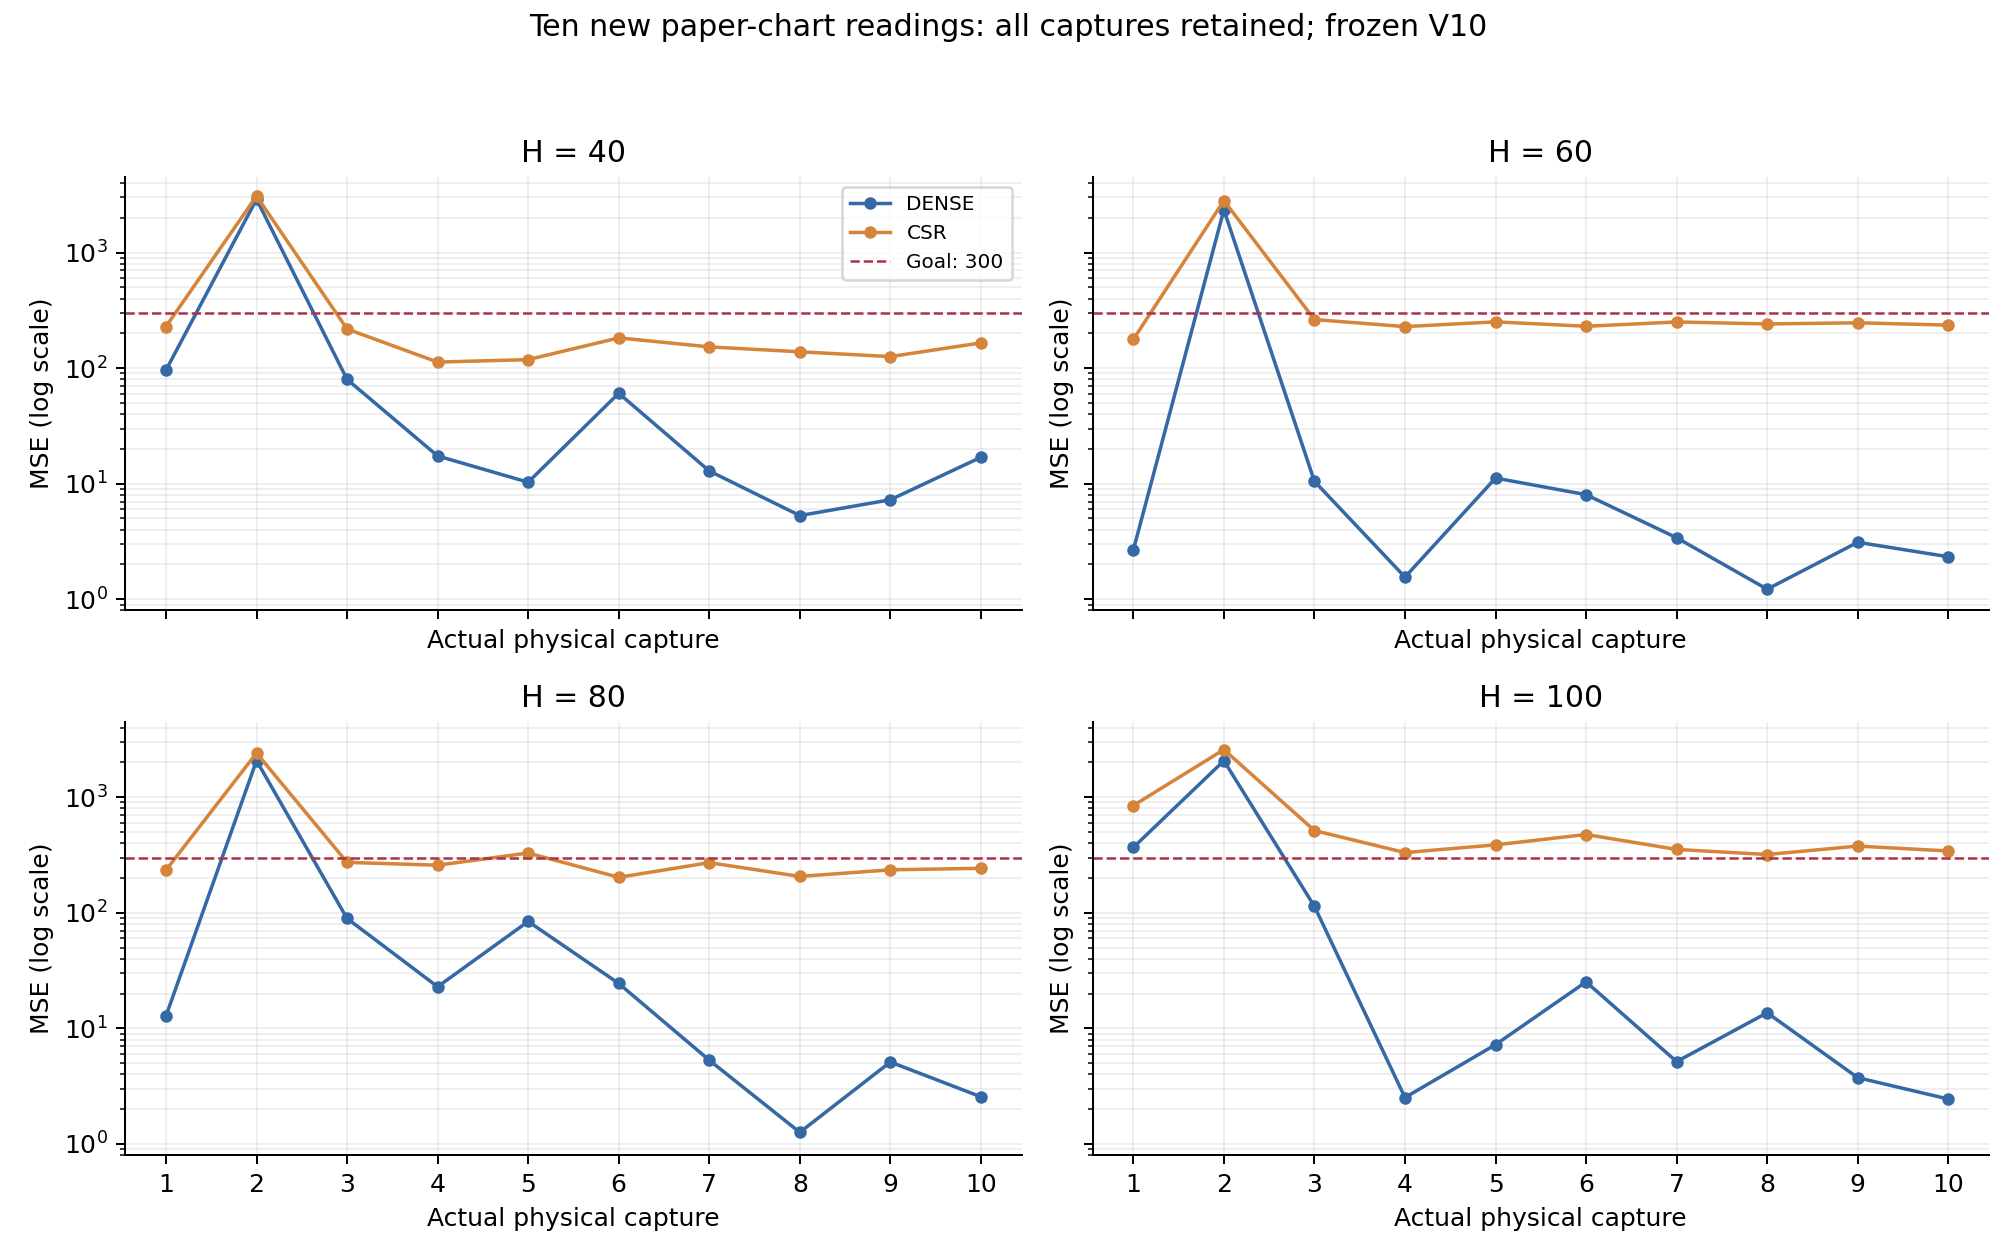
\includegraphics{figures/physical_mse10.png}

\begingroup\centering\setlength{\parindent}{0pt}

図2　各回のMSE（縦軸は対数目盛　破線は目標300）

\par\endgroup

\end{minipage}

\subsection{モデル配列容量}\label{ux30e2ux30c7ux30ebux914dux5217ux5bb9ux91cf}

\Needspace{10\baselineskip}

\begingroup\centering\setlength{\parindent}{0pt}

表3　枝刈り閾値と配列容量

\par\endgroup

\begin{longtable}[]{@{}lrrrrrr@{}}
\toprule\noalign{}
H & 閾値 & NNZ & 疎性 & Dense byte & CSR byte & 削減率 \\
\midrule\noalign{}
\endhead
\bottomrule\noalign{}
\endlastfoot
40 & 0.06084981 & 470 & 74.46\% & 7,692 & 2,854 & 62.90\% \\
60 & 0.05434179 & 1141 & 71.19\% & 16,332 & 6,449 & 60.51\% \\
80 & 0.04554720 & 1649 & 76.03\% & 28,172 & 9,229 & 67.24\% \\
100 & 0.05893202 & 2374 & 77.60\% & 43,212 & 13,094 & 69.70\% \\
\end{longtable}

NNZは非ゼロ重み数，疎性は重みを0にした割合を示す．全HでCSR索引を含む配列容量が減少した．最小容量はH40の2,854
byte，最大削減率はH100の69.70\%だった．

\subsection{実機推論時間}\label{ux5b9fux6a5fux63a8ux8ad6ux6642ux9593}

\Needspace{10\baselineskip}

\begingroup\centering\setlength{\parindent}{0pt}

表4　固定入力での推論時間（µs/推論）

\par\endgroup

\begin{longtable}[]{@{}lrrr@{}}
\toprule\noalign{}
H & Dense 平均±SD & CSR 平均±SD & 時間短縮率 \\
\midrule\noalign{}
\endhead
\bottomrule\noalign{}
\endlastfoot
40 & 465.262 ± 0.0179 & 305.834 ± 0.0913 & 34.27\% \\
60 & 945.648 ± 0.0217 & 671.674 ± 0.0799 & 28.97\% \\
80 & 1593.368 ± 0.0192 & 956.212 ± 0.2984 & 39.99\% \\
100 & 2408.160 ± 0.0158 & 1348.392 ± 0.2527 & 44.01\% \\
\end{longtable}

全Hで28.97〜44.01\%短縮した．表4の±は100推論の平均時間5組の標本SDであり，表1の読取10回のMSEのSDとは異なる．

\Needspace{18\baselineskip}

\noindent\begin{minipage}{\linewidth}

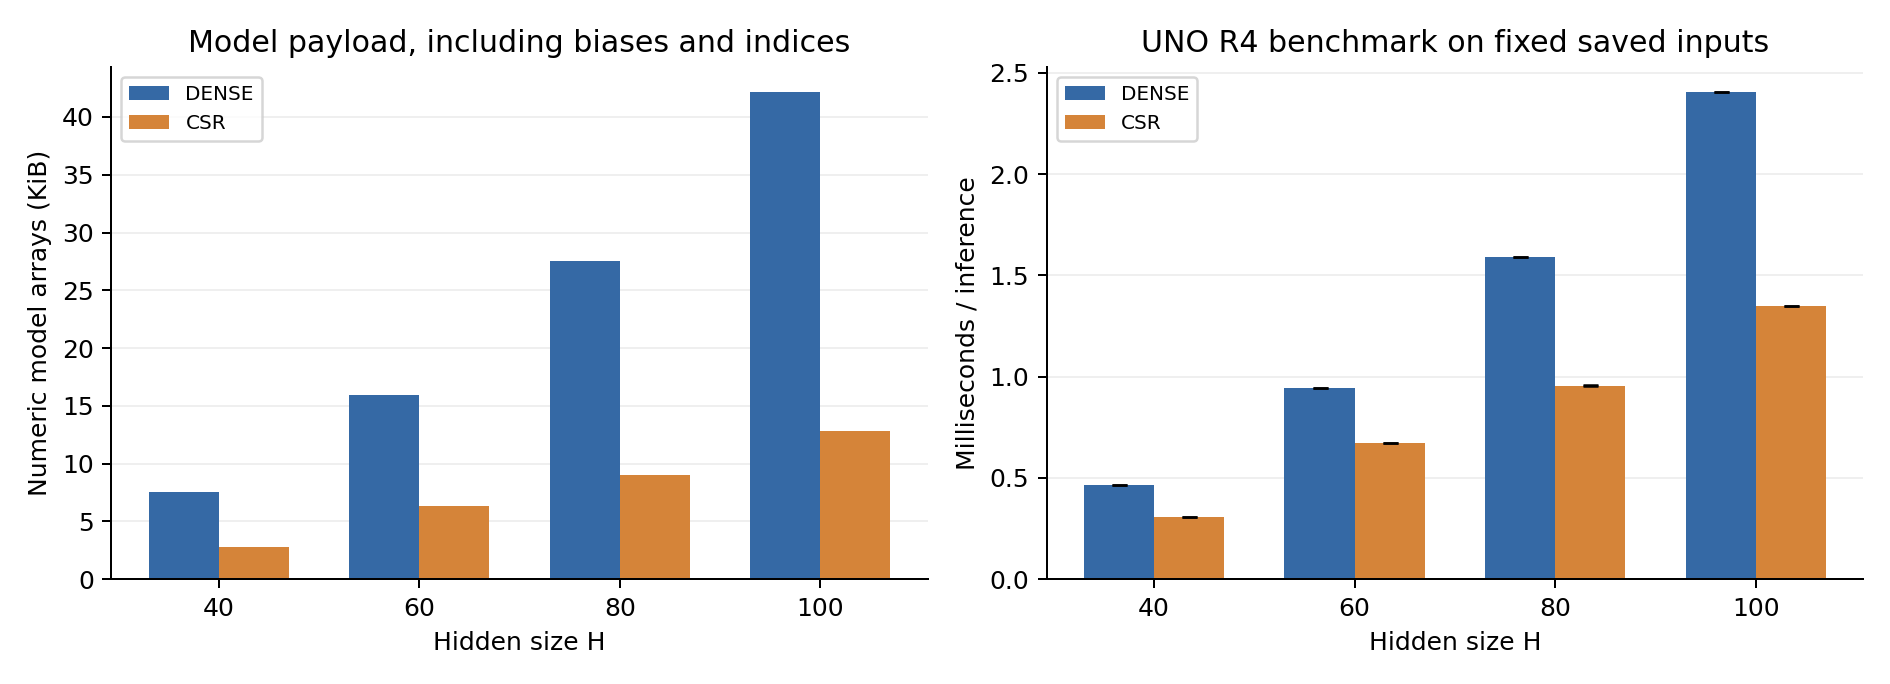
\includegraphics{figures/capacity_and_time.png}

\begingroup\centering\setlength{\parindent}{0pt}

図3　モデル配列容量と推論時間（誤差棒は5組の標本SD）

\par\endgroup

\end{minipage}

\Needspace{14\baselineskip}

\subsection{Flash・RAMと動作確認}\label{flashramux3068ux52d5ux4f5cux78baux8a8d}

\Needspace{10\baselineskip}

\begingroup\centering\setlength{\parindent}{0pt}

表5　8条件入りプログラム全体のArduino IDE使用量（byte）

\par\endgroup

\begin{longtable}[]{@{}lrrr@{}}
\toprule\noalign{}
プログラム & Flash & 静的RAM & 静的割当後の残りRAM \\
\midrule\noalign{}
\endhead
\bottomrule\noalign{}
\endlastfoot
保存入力再生・速度版 & 187,888 & 6,740 & 26,028 \\
新規読取版・全8条件 & 191,320 & 7,324 & 25,444 \\
\end{longtable}

\Needspace{10\baselineskip}

\begingroup\centering\setlength{\parindent}{0pt}

表6　単独モデル入りプログラムの使用量（byte）

\par\endgroup

\begin{longtable}[]{@{}lrrrrr@{}}
\toprule\noalign{}
H & Dense Flash & CSR Flash & Flash削減量 & 削減率 & 両方式の静的RAM \\
\midrule\noalign{}
\endhead
\bottomrule\noalign{}
\endlastfoot
40 & 60,852 & 56,020 & 4,832 & 7.94\% & 6,764 \\
60 & 69,492 & 59,612 & 9,880 & 14.22\% & 6,764 \\
80 & 81,348 & 62,396 & 18,952 & 23.30\% & 6,764 \\
100 & 96,388 & 66,260 & 30,128 & 31.26\% & 6,764 \\
\end{longtable}

条件名付きIDE表示に基づき，全HでFlashが減少した．H100では30,128
byte（31.26\%）削減した．静的RAMは全8条件で6,764
byte，静的割当後の残りは26,004 byteだった．

\Needspace{19\baselineskip}

\noindent\begin{minipage}{\linewidth}

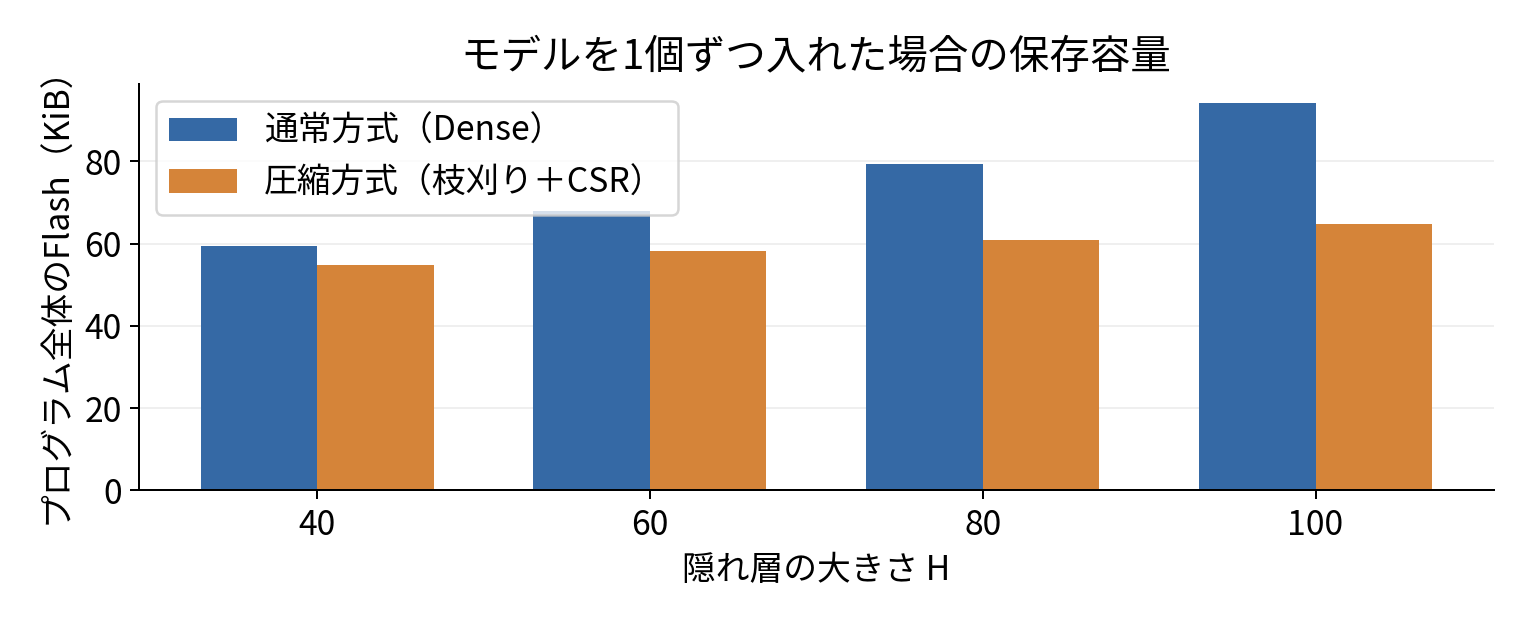
\includegraphics{figures/single_model_flash.png}

\begingroup\centering\setlength{\parindent}{0pt}

図4　単独モデルのFlash使用量

\par\endgroup

\end{minipage}

Flash全体はArduinoコア等を含み，モデル配列だけの削減率とは異なる．モデルはconst配列であり，関数内の中間配列も静的RAMには含まれない．残り26,004
byteはローカル変数の実使用量ではない．中間配列はfloat{[}100{]}を2本，宣言上800
byteだが，実行時スタックの最大量は未測定である．

保存入力版の実機自己検査とCSR索引検査はPASSした．新規10回の全80PPM，計2,160
RGB成分は固定V10のPC再計算と一致した．80個のMSEは先生の元の計算HTMLとも表示桁の範囲で一致した．

\section{考察}\label{ux8003ux5bdf}

\subsection{容量・速度と精度の両立}\label{ux5bb9ux91cfux901fux5ea6ux3068ux7cbeux5ea6ux306eux4e21ux7acb}

検証128入力ではMSE増加5\%以下を満たしたが，新規10回では満たさなかった．入力が同じ0へ潰れる問題や読取状態の変動が考えられるものの，支配的な要因は特定できない．今回の閾値では，枝刈りによる出力への影響を十分小さくできなかった．

\subsection{メモリ・速度・推論性能の定量的な対応}\label{ux30e1ux30e2ux30eaux901fux5ea6ux63a8ux8ad6ux6027ux80fdux306eux5b9aux91cfux7684ux306aux5bfeux5fdc}

H60で3つの指標を合わせて考える．まず容量は，モデル配列が16,332→6,449
byteで60.51\%減った．プログラム全体のFlashは69,492→59,612
byteで14.22\%減った．Arduinoの共通処理などが残るため，モデルだけの削減率とプログラム全体の削減率は違う．静的RAMは6,764→6,764
byteで0\%削減だった．

次に速度を考える．重みと入力を掛ける回数は，通常方式で \(N_w=H^2+6H\)
回，圧縮方式でK回になる．H60では3,960→1,141回で71.19\%減ったが，計算時間の短縮は945.648→671.674
µsで28.97\%だった．

掛け算の回数ほど時間が減らないのは，位置情報を読む処理や繰り返し処理なども必要だからである．全Hでも掛け算の回数は71.19〜77.60\%減ったのに対し，時間は28.97〜44.01\%の短縮だった．各処理の時間を別々に測ってはいないため，どの処理に最も時間がかかったかは断定しない．

一方，H60の新規10回平均MSEは238.33→493.51で，255.17増加した．差の標本SDは79.33であり，同じ回の対応差は10回とも正だった．H40でもFlashは7.94\%，時間は34.27\%減ったが，平均MSEは319.56→452.04で41.46\%増えた．したがって，容量・速度の改善と精度維持を同時に満たした条件は今回の4組にはなかった．

\subsection{第2回とばらつき}\label{ux7b2c2ux56deux3068ux3070ux3089ux3064ux304d}

第2回は全モデルでMSEが大きく，平均とSDに強く影響した．H60のDenseは最小1.22，最大2,339.37，平均238.33，標本SD738.23だった．

青・水色などのRAW・正規化入力も他の回と異なった．PCと実機の出力は一致しているため，MSE表示だけの差ではない．校正・照射・紙の位置・センサ応答が原因候補だが，照度や距離の記録がなく断定できない．操作ミスの申告もなかったため第2回を保持した．

\subsection{次元数と評価の限界}\label{ux6b21ux5143ux6570ux3068ux8a55ux4fa1ux306eux9650ux754c}

Denseの平均MSEはH80で最小だったが，Hの増加に対して単調には改善しなかった．Hごとに初期重みも異なり，H単独の効果とは断定できない．H40のCSRは最小容量・最短時間，H100は最大削減率・時間短縮率だったが，精度維持を同時に満たした条件はなかった．

測定は手持ちの同一チャートを続けて10回読んだものであり，距離・角度・照度は定量統制していない．独立最終チャート，H50，各方式の搭載限界，最大スタック使用量は未測定である．学習損失，学習行を再入力したMSE，新規読取のMSEは分けて解釈する．

\subsection{今後の改善}\label{ux4ecaux5f8cux306eux6539ux5584}

まず閾値を下げ，層別の閾値選択と，削除接続を0に固定した再学習を検討する．設定は検証データで選び，固定後に別の最終チャートでMSE300以下と増加5\%以下を判定する．

検証128入力には，異なる6色が同じ(0,0,0)になる入力衝突があった．RAW・クリップ前入力・飽和割合と校正変動を記録し，情報が失われる段階を調べる．照明・距離・角度の変動を定量化し，対応範囲を学習に反映する．

中間配列を各Hに合わせれば宣言上800 byteから \(8H\)
byteへ削減でき，H40では320
byteとなる．これは未実装の案である．リンカマップと最大スタック量を記録し，整数索引の上限も含めて搭載限界を調べる．入力選択・チェックサムを分離した計時も追加する．

H50を補い，seed・測定日を変えた反復と独立チャートによる評価を行う．H200への拡張はメモリと索引の範囲を確認してから実施する．

\section{結論}\label{ux7d50ux8ad6}

H40・60・80・100の枝刈り＋CSRは，Denseに対しモデル配列容量を60.51〜69.70\%，固定入力での実機推論時間を28.97〜44.01\%，単独ビルドのFlashを7.94〜31.26\%削減した．静的RAMは全条件で6,764
byteと変わらなかった．

一方，新規10回の平均MSEは全Hで増加し，MSE増加5\%以下とCSRの平均MSE300以下は達成しなかった．容量・速度の改善は確認したが，精度維持との両立には，入力の再現性，閾値選択，枝刈り後の再学習を見直し，独立チャートで検証する必要がある．

\section{参考文献}\label{ux53c2ux8003ux6587ux732e}

{[}1{]} R. Tibshirani， ``Regression Shrinkage and Selection via the
Lasso，'' Journal of the Royal Statistical Society: Series B， 58(1)，
pp.~267--288， 1996．

{[}2{]} S. Han， J. Pool， J. Tran， and W. J. Dally， ``Learning Both
Weights and Connections for Efficient Neural Networks，'' Advances in
Neural Information Processing Systems 28， pp.~1135--1143， 2015．

{[}3{]} N. Bell and M. Garland， ``Implementing Sparse Matrix-Vector
Multiplication on Throughput-Oriented Processors，'' Proceedings of SC
'09， Article 18， pp.~1--11， 2009．

{[}4{]} Arduino， ``micros()，'' Arduino Documentation，
\url{https://docs.arduino.cc/language-reference/en/functions/time/micros/}．

{[}5{]} PyTorch Contributors， ``SmoothL1Loss，'' PyTorch
Documentation，
\url{https://docs.pytorch.org/docs/stable/generated/torch.nn.SmoothL1Loss.html}．

\section{付録：各回の実測値と再現資料}\label{ux4ed8ux9332ux5404ux56deux306eux5b9fux6e2cux5024ux3068ux518dux73feux8cc7ux6599}

\Needspace{16\baselineskip}

\subsection{全10回のDense MSE}\label{ux516810ux56deux306edense-mse}

\begin{longtable}[]{@{}lrrrr@{}}
\toprule\noalign{}
回 & H40 & H60 & H80 & H100 \\
\midrule\noalign{}
\endhead
\bottomrule\noalign{}
\endlastfoot
1 & 96.03 & 2.66 & 12.77 & 367.18 \\
2 & 2889.14 & 2339.37 & 2069.25 & 2063.62 \\
3 & 79.85 & 10.48 & 89.18 & 113.51 \\
4 & 17.37 & 1.55 & 22.88 & 2.51 \\
5 & 10.29 & 11.18 & 84.03 & 7.22 \\
6 & 60.55 & 8.03 & 24.44 & 25.22 \\
7 & 12.88 & 3.40 & 5.29 & 5.14 \\
8 & 5.29 & 1.22 & 1.25 & 13.62 \\
9 & 7.25 & 3.11 & 5.11 & 3.74 \\
10 & 16.92 & 2.33 & 2.55 & 2.44 \\
\end{longtable}

\Needspace{16\baselineskip}

\subsection{全10回の枝刈り＋CSR
MSE}\label{ux516810ux56deux306eux679dux5208ux308acsr-mse}

\begin{longtable}[]{@{}lrrrr@{}}
\toprule\noalign{}
回 & H40 & H60 & H80 & H100 \\
\midrule\noalign{}
\endhead
\bottomrule\noalign{}
\endlastfoot
1 & 228.85 & 177.18 & 233.81 & 846.00 \\
2 & 3078.33 & 2811.55 & 2407.85 & 2576.07 \\
3 & 217.77 & 262.88 & 272.62 & 513.88 \\
4 & 112.70 & 228.59 & 257.70 & 331.37 \\
5 & 118.37 & 251.22 & 328.44 & 386.29 \\
6 & 182.55 & 230.07 & 202.44 & 474.85 \\
7 & 152.55 & 250.62 & 271.07 & 352.70 \\
8 & 138.37 & 241.03 & 206.03 & 318.85 \\
9 & 125.74 & 246.51 & 235.03 & 377.07 \\
10 & 165.14 & 235.40 & 242.25 & 342.18 \\
\end{longtable}

\subsection{学習135行の重みなしMSE}\label{ux5b66ux7fd2135ux884cux306eux91cdux307fux306aux3057mse}

全行の重要度を等しくしたMSEを示す．学習損失や新規10回のMSEとは異なる．

\begin{longtable}[]{@{}lrr@{}}
\toprule\noalign{}
H & 学習135行のMSE & うち3×3の111行のMSE \\
\midrule\noalign{}
\endhead
\bottomrule\noalign{}
\endlastfoot
40 & 1794.73 & 1049.09 \\
60 & 1346.71 & 867.25 \\
80 & 1151.08 & 764.49 \\
100 & 922.76 & 495.81 \\
\end{longtable}

使用コード・集計CSV・元ログと再計算手順は同梱READMEに，各ファイルのSHA256は
\texttt{manifest.json} に示す．

\subsection{コメント付きコード}\label{ux30b3ux30e1ux30f3ux30c8ux4ed8ux304dux30b3ux30fcux30c9}

実際に使用した \texttt{teacher\_compare\_v10.ino}
の関数に，行ごとの説明コメントを加えて示す．

\Needspace{22\baselineskip}

\subsubsection{CSR層の推論}\label{csrux5c64ux306eux63a8ux8ad6}

\begin{Shaded}
\begin{Highlighting}[]
\DataTypeTok{void}\NormalTok{ sparseLayer}\OperatorTok{(} \CommentTok{// CSR形式の1層を計算する関数}
  \AttributeTok{const}\NormalTok{ comparison\_models}\OperatorTok{::}\NormalTok{SparseLayer }\OperatorTok{\&}\NormalTok{layer}\OperatorTok{,} \CommentTok{// 層の重みと位置情報}
  \AttributeTok{const} \DataTypeTok{float} \OperatorTok{*}\NormalTok{input}\OperatorTok{,} \CommentTok{// 入力配列を受け取る}
  \DataTypeTok{float} \OperatorTok{*}\NormalTok{output}\OperatorTok{,} \CommentTok{// 計算結果を書き込む配列}
  \DataTypeTok{bool}\NormalTok{ relu }\CommentTok{// ReLUを適用するかの指定}
\OperatorTok{)} \OperatorTok{\{} \CommentTok{// 関数の処理を開始する}
  \ControlFlowTok{for} \OperatorTok{(}\DataTypeTok{int}\NormalTok{ r }\OperatorTok{=} \DecValTok{0}\OperatorTok{;}\NormalTok{ r }\OperatorTok{\textless{}}\NormalTok{ layer}\OperatorTok{.}\NormalTok{rows}\OperatorTok{;}\NormalTok{ r}\OperatorTok{++)} \OperatorTok{\{} \CommentTok{// 出力先の各行を順に計算する}
    \DataTypeTok{float}\NormalTok{ value }\OperatorTok{=}\NormalTok{ layer}\OperatorTok{.}\NormalTok{bias}\OperatorTok{[}\NormalTok{r}\OperatorTok{];} \CommentTok{// その行のバイアスを合計の初期値にする}
    \ControlFlowTok{for} \OperatorTok{(}\DataTypeTok{uint16\_t}\NormalTok{ k }\OperatorTok{=}\NormalTok{ layer}\OperatorTok{.}\NormalTok{row}\OperatorTok{[}\NormalTok{r}\OperatorTok{];} \CommentTok{// その行の非ゼロ重みの開始位置}
\NormalTok{         k }\OperatorTok{\textless{}}\NormalTok{ layer}\OperatorTok{.}\NormalTok{row}\OperatorTok{[}\NormalTok{r}\OperatorTok{+}\DecValTok{1}\OperatorTok{];} \CommentTok{// 次の行の開始位置の手前まで繰り返す}
\NormalTok{         k}\OperatorTok{++)} \CommentTok{// 次の保存位置へ進む}
\NormalTok{      value }\OperatorTok{+=}\NormalTok{ layer}\OperatorTok{.}\NormalTok{values}\OperatorTok{[}\NormalTok{k}\OperatorTok{]} \OperatorTok{*}\NormalTok{ input}\OperatorTok{[}\NormalTok{layer}\OperatorTok{.}\NormalTok{col}\OperatorTok{[}\NormalTok{k}\OperatorTok{]];} \CommentTok{// 重みと対応入力の積を加える}
\NormalTok{    output}\OperatorTok{[}\NormalTok{r}\OperatorTok{]} \OperatorTok{=} \OperatorTok{(}\NormalTok{relu }\OperatorTok{\&\&}\NormalTok{ value }\OperatorTok{\textless{}} \DecValTok{0}\OperatorTok{)} \OperatorTok{?} \DecValTok{0} \OperatorTok{:}\NormalTok{ value}\OperatorTok{;} \CommentTok{// 指定時は負の値を0にする}
  \OperatorTok{\}} \CommentTok{// その行の計算を終える}
\OperatorTok{\}} \CommentTok{// 関数を終える}
\end{Highlighting}
\end{Shaded}

\Needspace{27\baselineskip}

\subsubsection{推論時間の計測}\label{ux63a8ux8ad6ux6642ux9593ux306eux8a08ux6e2c}

\begin{Shaded}
\begin{Highlighting}[]
\DataTypeTok{uint32\_t}\NormalTok{ timeModel}\OperatorTok{(} \CommentTok{// 100推論の経過時間を返す関数}
  \DataTypeTok{int}\NormalTok{ model}\OperatorTok{,} \CommentTok{// 計時するモデルの番号}
  \DataTypeTok{int}\NormalTok{ group}\OperatorTok{,} \CommentTok{// 計時する組の番号}
  \DataTypeTok{double} \OperatorTok{\&}\NormalTok{checksum }\CommentTok{// 出力の合計を呼出元へ返す参照}
\OperatorTok{)} \OperatorTok{\{} \CommentTok{// 関数の処理を開始する}
  \DataTypeTok{float}\NormalTok{ output}\OperatorTok{[}\DecValTok{3}\OperatorTok{];} \CommentTok{// 推論結果のRGBを一時保存する}
\NormalTok{  checksum }\OperatorTok{=} \DecValTok{0}\OperatorTok{;} \CommentTok{// 出力の合計を初期化する}
  \DataTypeTok{uint32\_t}\NormalTok{ begin }\OperatorTok{=} \KeywordTok{static\_cast}\OperatorTok{\textless{}}\DataTypeTok{uint32\_t}\OperatorTok{\textgreater{}(}\NormalTok{micros}\OperatorTok{());} \CommentTok{// 開始時刻を記録する}
  \ControlFlowTok{for} \OperatorTok{(}\DataTypeTok{int}\NormalTok{ call }\OperatorTok{=} \DecValTok{0}\OperatorTok{;}\NormalTok{ call }\OperatorTok{\textless{}} \DecValTok{100}\OperatorTok{;}\NormalTok{ call}\OperatorTok{++)} \OperatorTok{\{} \CommentTok{// 100回の推論を繰り返す}
    \DataTypeTok{int}\NormalTok{ input }\OperatorTok{=} \OperatorTok{(}\NormalTok{group }\OperatorTok{*} \DecValTok{100} \OperatorTok{+}\NormalTok{ call}\OperatorTok{)} \CommentTok{// 組を通した呼出番号を求める}
      \OperatorTok{\%}\NormalTok{ comparison\_models}\OperatorTok{::}\NormalTok{BENCHMARK\_INPUT\_COUNT}\OperatorTok{;} \CommentTok{// 9入力を巡回する番号にする}
\NormalTok{    comparison\_models}\OperatorTok{::}\NormalTok{predict}\OperatorTok{(} \CommentTok{// 指定モデルの推論を呼び出す}
\NormalTok{      model}\OperatorTok{,} \CommentTok{// モデル番号を渡す}
\NormalTok{      comparison\_models}\OperatorTok{::}\NormalTok{BENCHMARK\_INPUTS}\OperatorTok{[}\NormalTok{input}\OperatorTok{],} \CommentTok{// 選んだ保存入力を渡す}
\NormalTok{      output}\OperatorTok{);} \CommentTok{// 結果をoutputに受け取る}
\NormalTok{    checksum }\OperatorTok{+=}\NormalTok{ output}\OperatorTok{[}\DecValTok{0}\OperatorTok{]} \OperatorTok{+}\NormalTok{ output}\OperatorTok{[}\DecValTok{1}\OperatorTok{]} \OperatorTok{+}\NormalTok{ output}\OperatorTok{[}\DecValTok{2}\OperatorTok{];} \CommentTok{// RGBの出力を合計へ加える}
  \OperatorTok{\}} \CommentTok{// 100回の繰り返しを終える}
  \ControlFlowTok{return} \KeywordTok{static\_cast}\OperatorTok{\textless{}}\DataTypeTok{uint32\_t}\OperatorTok{\textgreater{}(}\NormalTok{micros}\OperatorTok{())} \OperatorTok{{-}}\NormalTok{ begin}\OperatorTok{;} \CommentTok{// 経過時間をµsで返す}
\OperatorTok{\}} \CommentTok{// 関数を終える}
\end{Highlighting}
\end{Shaded}


\end{document}
